\documentclass[11pt,letterpaper]{article}

\usepackage[margin=0.85in]{geometry}
\usepackage{amsmath,amssymb,amsthm}
\usepackage{booktabs}
\usepackage{graphicx}
\usepackage{microtype}
\usepackage{xcolor}
\usepackage{enumitem}
\usepackage{array}
\usepackage{listings}
\usepackage[colorlinks=true,linkcolor=blue!60!black,citecolor=blue!60!black,urlcolor=blue!60!black]{hyperref}

\theoremstyle{plain}
\newtheorem{theorem}{Theorem}
\newtheorem{corollary}{Corollary}
\newtheorem{proposition}{Proposition}
\newtheorem{lemma}{Lemma}

\theoremstyle{definition}
\newtheorem{definition}{Definition}

\theoremstyle{remark}
\newtheorem{remark}{Remark}

\newcommand{\F}{\mathbb{F}}
\newcommand{\Z}{\mathbb{Z}}
\newcommand{\wt}{\mathrm{wt}}

\lstset{
  basicstyle=\ttfamily\scriptsize,
  breaklines=true,
  frame=single,
  rulecolor=\color{black!25},
  backgroundcolor=\color{black!3},
  xleftmargin=4pt,
  xrightmargin=4pt
}

% AUTO-GENERATED by scripts/generate_bt011_paper_assets.py — DO NOT EDIT MANUALLY

\newcommand{\TableAllThirtySixRecords}{
\begin{table*}[t]
\centering
\caption{All thirty-six (36) improved binary constant-weight code lower bounds strictly exceeding Andries~E.\ Brouwer's live November~24, 2026 (\texttt{22:50 CET}) table~\cite{BrouwerAndw} across $24 \le n \le 30$ and $7 \le w \le 15$, including every listed cell at $n = 25$ ($6/6$) and $n = 30$ ($9/9$). ``Nested Johnson UB'' denotes the recursive floor bound of~\eqref{eq:johnson} (for $A(27,4,13)$, complement symmetry with $w=14$ tightens this slightly to $1{,}322{,}394$). Every code is independently verified with zero $(w{-}1)$-subset collisions in compiled Go and bit-exact SHA-256 parity ($\mathrm{Go} = \mathrm{Python}$) in our zero-shared-code pure-Python verifier (WOF-1 composite SHA-256: \texttt{ff6475f8763defd1...}).}
\label{tab:all36}
\scriptsize
\setlength{\tabcolsep}{3.6pt}
\renewcommand{\arraystretch}{0.96}
\resizebox{\textwidth}{!}{%
\begin{tabular}{@{}r l c r r r r r r c@{}}
\toprule
\# & Cell & Split $(n_1{+}n_2, p)$ & Prior LB & \textbf{New LB} & \textbf{Gain} & Nested Johnson UB & $(w{-}1)$-Subtuples ($0$ coll.) & Explicit $O(M^2)$ Pairs & SHA-256 (12) \\
\midrule
1 & $A(24,4,11)$ & $12+12$ (even) & $118{,}422\,\mathrm{p}$ & $\mathbf{118{,}430}$ & $\mathbf{+8}$ & $164{,}565$ & $1{,}302{,}730$ & --- & \texttt{353dad33f049} \\
\addlinespace[1.8pt]
2 & $A(25,4,7)$ & $12+13$ (even) & $21{,}220\,\mathrm{p}$ & $\mathbf{21{,}226}$ & $\mathbf{+6}$ & $25{,}300$ & $148{,}582$ & $225{,}260{,}925$ & \texttt{7e7d6d8324ee} \\
3 & $A(25,4,8)$ & $12+13$ (odd) & $47{,}265\,\mathrm{p}$ & $\mathbf{47{,}285}$ & $\mathbf{+20}$ & $56{,}925$ & $378{,}280$ & $1{,}117{,}911{,}970$ & \texttt{d19ef03db0bb} \\
4 & $A(25,4,9)$ & $12+13$ (even) & $89{,}742\,\mathrm{p}$ & $\mathbf{89{,}748}$ & $\mathbf{+6}$ & $120{,}175$ & $807{,}732$ & --- & \texttt{ab9193e97817} \\
5 & $A(25,4,10)$ & $12+13$ (even) & $142{,}373\,\mathrm{p}$ & $\mathbf{142{,}397}$ & $\mathbf{+24}$ & $192{,}280$ & $1{,}423{,}970$ & --- & \texttt{5031aa413e3a} \\
6 & $A(25,4,11)$ & $12+13$ (even) & $198{,}387\,\mathrm{p}$ & $\mathbf{198{,}425}$ & $\mathbf{+38}$ & $293{,}938$ & $2{,}182{,}675$ & --- & \texttt{c2f98eef358b} \\
7 & $A(25,4,12)$ & $12+13$ (even) & $231{,}530\,\mathrm{p}$ & $\mathbf{231{,}554}$ & $\mathbf{+24}$ & $342{,}843$ & $2{,}778{,}648$ & --- & \texttt{892bd8f29bf5} \\
\addlinespace[1.8pt]
8 & $A(26,4,8)$ & $13+13$ (odd) & $66{,}352\,\mathrm{p}$ & $\mathbf{66{,}404}$ & $\mathbf{+52}$ & $82{,}225$ & $531{,}232$ & $2{,}204{,}712{,}406$ & \texttt{43dc30ea3fe5} \\
9 & $A(26,4,9)$ & $13+13$ (even) & $129{,}708\,\mathrm{p}$ & $\mathbf{129{,}734}$ & $\mathbf{+26}$ & $164{,}450$ & $1{,}167{,}606$ & --- & \texttt{ce929a32467b} \\
10 & $A(26,4,10)$ & $13+13$ (odd) & $222{,}775\,\mathrm{p}$ & $\mathbf{222{,}827}$ & $\mathbf{+52}$ & $312{,}455$ & $2{,}228{,}270$ & --- & \texttt{8e410a7f0f08} \\
11 & $A(26,4,11)$ & $13+13$ (even) & $320{,}584\,\mathrm{p}$ & $\mathbf{320{,}610}$ & $\mathbf{+26}$ & $454{,}480$ & $3{,}526{,}710$ & --- & \texttt{7bacc232fec0} \\
12 & $A(26,4,12)$ & $12+14$ (even) & $401{,}937\,\mathrm{p}$ & $\mathbf{402{,}141}$ & $\mathbf{+204}$ & $636{,}865$ & $4{,}825{,}692$ & --- & \texttt{c8f1d661b776} \\
\addlinespace[1.8pt]
13 & $A(27,4,9)$ & $13+14$ (odd) & $188{,}561\,\mathrm{p}$ & $\mathbf{188{,}795}$ & $\mathbf{+234}$ & $246{,}675$ & $1{,}699{,}155$ & --- & \texttt{44360951d541} \\
14 & $A(27,4,10)$ & $13+14$ (even) & $334{,}859\,\mathrm{p}$ & $\mathbf{334{,}868}$ & $\mathbf{+9}$ & $444{,}015$ & $3{,}348{,}680$ & --- & \texttt{037fa763a05d} \\
15 & $A(27,4,11)$ & $13+14$ (odd) & $518{,}014\,\mathrm{p}$ & $\mathbf{518{,}269}$ & $\mathbf{+255}$ & $766{,}935$ & $5{,}700{,}959$ & --- & \texttt{b959715ed60d} \\
16 & $A(27,4,12)$ & $13+14$ (even) & $686{,}164\,\mathrm{p}$ & $\mathbf{686{,}227}$ & $\mathbf{+63}$ & $1{,}022{,}580$ & $8{,}234{,}724$ & --- & \texttt{acbb1d4516e4} \\
17 & $A(27,4,13)$ & $13+14$ (odd) & $791{,}461\,\mathrm{p}$ & $\mathbf{791{,}536}$ & $\mathbf{+75}$ & $1{,}322{,}719$ & $10{,}289{,}968$ & --- & \texttt{9c5f3d0f9dcf} \\
\addlinespace[1.8pt]
18 & $A(28,4,7)$ & $14+14$ (even) & $44{,}915\,\mathrm{p}$ & $\mathbf{44{,}929}$ & $\mathbf{+14}$ & $51{,}480$ & $314{,}503$ & $1{,}009{,}285{,}056$ & \texttt{e72d0d0e610e} \\
19 & $A(28,4,10)$ & $14+14$ (even) & $508{,}952\,\mathrm{p}$ & $\mathbf{508{,}998}$ & $\mathbf{+46}$ & $690{,}690$ & $5{,}089{,}980$ & --- & \texttt{6fe83acc011b} \\
20 & $A(28,4,11)$ & $14+14$ (even) & $819{,}041\,\mathrm{p}$ & $\mathbf{819{,}084}$ & $\mathbf{+43}$ & $1{,}130{,}220$ & $9{,}009{,}924$ & --- & \texttt{8040bfd7269c} \\
21 & $A(28,4,12)$ & $14+14$ (even) & $1{,}167{,}909\,\mathrm{p}$ & $\mathbf{1{,}167{,}955}$ & $\mathbf{+46}$ & $1{,}789{,}515$ & $14{,}015{,}460$ & --- & \texttt{3c8983ae1a0e} \\
\addlinespace[1.8pt]
22 & $A(29,4,8)$ & $13+16$ (even) & $157{,}734\,\mathrm{p}$ & $\mathbf{157{,}889}$ & $\mathbf{+155}$ & $186{,}615$ & $1{,}263{,}112$ & --- & \texttt{58f683baad89} \\
23 & $A(29,4,9)$ & $13+16$ (odd) & $365{,}699\,\mathrm{p}$ & $\mathbf{366{,}191}$ & $\mathbf{+492}$ & $475{,}020$ & $3{,}295{,}719$ & --- & \texttt{c71bbf737d88} \\
24 & $A(29,4,11)$ & $14+15$ (even) & $1{,}266{,}026\,\mathrm{p}$ & $\mathbf{1{,}266{,}111}$ & $\mathbf{+85}$ & $1{,}820{,}910$ & $13{,}927{,}221$ & --- & \texttt{0bcd7db3ea5a} \\
25 & $A(29,4,12)$ & $13+16$ (even) & $1{,}895{,}939\,\mathrm{p}$ & $\mathbf{1{,}896{,}915}$ & $\mathbf{+976}$ & $2{,}731{,}365$ & $22{,}762{,}980$ & --- & \texttt{7db3dc78ea43} \\
26 & $A(29,4,13)$ & $13+16$ (odd) & $2{,}499{,}311\,\mathrm{p}$ & $\mathbf{2{,}500{,}447}$ & $\mathbf{+1{,}136}$ & $3{,}991{,}995$ & $32{,}505{,}811$ & --- & \texttt{fb392b76730b} \\
27 & $A(29,4,14)$ & $13+16$ (even) & $2{,}870{,}880\,\mathrm{p}$ & $\mathbf{2{,}872{,}206}$ & $\mathbf{+1{,}326}$ & $4{,}562{,}280$ & $40{,}210{,}884$ & --- & \texttt{0516135b9d96} \\
\addlinespace[1.8pt]
28 & $A(30,4,7)$ & $14+16$ (odd) & $73{,}853\,\mathrm{p}$ & $\mathbf{74{,}077}$ & $\mathbf{+224}$ & $81{,}424$ & $518{,}539$ & $2{,}743{,}663{,}926$ & \texttt{8887a8d875cb} \\
29 & $A(30,4,8)$ & $14+16$ (even) & $214{,}545\,\mathrm{p}$ & $\mathbf{214{,}872}$ & $\mathbf{+327}$ & $254{,}475$ & $1{,}718{,}976$ & --- & \texttt{29f906a27222} \\
30 & $A(30,4,9)$ & $14+16$ (odd) & $514{,}015\,\mathrm{p}$ & $\mathbf{514{,}169}$ & $\mathbf{+154}$ & $622{,}050$ & $4{,}627{,}521$ & --- & \texttt{c2d768eca554} \\
31 & $A(30,4,10)$ & $14+16$ (even) & $1{,}085{,}000\,\mathrm{p}$ & $\mathbf{1{,}086{,}033}$ & $\mathbf{+1{,}033}$ & $1{,}425{,}060$ & $10{,}860{,}330$ & --- & \texttt{eade92da40cd} \\
32 & $A(30,4,11)$ & $14+16$ (odd) & $1{,}977{,}548\,\mathrm{p}$ & $\mathbf{1{,}979{,}156}$ & $\mathbf{+1{,}608}$ & $2{,}584{,}516$ & $21{,}770{,}716$ & --- & \texttt{17adf085863f} \\
33 & $A(30,4,12)$ & $14+16$ (even) & $3{,}143{,}989\,\mathrm{p}$ & $\mathbf{3{,}145{,}679}$ & $\mathbf{+1{,}690}$ & $4{,}552{,}275$ & $37{,}748{,}148$ & --- & \texttt{19f188f0dbd1} \\
34 & $A(30,4,13)$ & $14+16$ (odd) & $4{,}325{,}235\,\mathrm{p}$ & $\mathbf{4{,}326{,}477}$ & $\mathbf{+1{,}242}$ & $6{,}303{,}150$ & $56{,}244{,}201$ & --- & \texttt{db66afb49177} \\
35 & $A(30,4,14)$ & $14+16$ (even) & $5{,}313{,}399\,\mathrm{p}$ & $\mathbf{5{,}315{,}657}$ & $\mathbf{+2{,}258}$ & $8{,}554{,}275$ & $74{,}419{,}198$ & --- & \texttt{f75b21581610} \\
36 & $A(30,4,15)$ & $14+16$ (odd) & $5{,}697{,}080\,\mathrm{p}$ & $\mathbf{5{,}699{,}800}$ & $\mathbf{+2{,}720}$ & $9{,}124{,}560$ & $85{,}497{,}000$ & --- & \texttt{e142a4514e65} \\
\midrule
\multicolumn{2}{@{}l}{\textbf{Total (36 cells)}} & 9 splits & $38{,}450{,}424$ & $\mathbf{38{,}467{,}121}$ & $\mathbf{+16{,}697}$ & $57{,}581{,}300$ & $\mathbf{486{,}375{,}836}$ & $\mathbf{7{,}300{,}834{,}283}$ & \texttt{ff6475f8763d} \\
\bottomrule
\end{tabular}%
}
\end{table*}
}

\newcommand{\TableCleanSweepSummary}{
\begin{table}[t]
\centering
\caption{Per-length aggregation of our 36 improved lower bounds across $24 \le n \le 30$, showing the 6/6 sweep of $n = 25$ and 9/9 sweep of $n = 30$ (which alone contributes $+11{,}256$ new codewords, $67.4\%$ of the total gain).}
\label{tab:sweep}
\scriptsize
\setlength{\tabcolsep}{4.5pt}
\resizebox{\textwidth}{!}{%
\begin{tabular}{@{}c c l r r r r@{}}
\toprule
Length $n$ & Improved / Listed ($w \ge 7$) & Weights $w$ Improved & Dominant Split(s) & \textbf{Total Gain} & Verified Codewords & $(w{-}1)$-Subtuples \\
\midrule
$24$ & 1/6 & $11$ & $12+12$ & $\mathbf{+8}$ & $118{,}430$ & $1{,}302{,}730$ \\
$25$ & 6/6 (\textbf{sweep}) & $7..12$ & $12+13$ & $\mathbf{+118}$ & $730{,}635$ & $7{,}719{,}887$ \\
$26$ & 5/7 & $8..12$ & $12+14$, $13+13$ & $\mathbf{+360}$ & $1{,}141{,}716$ & $12{,}279{,}510$ \\
$27$ & 5/7 & $9..13$ & $13+14$ & $\mathbf{+636}$ & $2{,}519{,}695$ & $29{,}273{,}486$ \\
$28$ & 4/8 & $7,10,11,12$ & $14+14$ & $\mathbf{+149}$ & $2{,}540{,}966$ & $28{,}429{,}867$ \\
$29$ & 6/8 & $8,9,11,12,13,14$ & $13+16$, $14+15$ & $\mathbf{+4{,}170}$ & $9{,}059{,}759$ & $113{,}965{,}727$ \\
$30$ & 9/9 (\textbf{sweep}) & $7..15$ & $14+16$ & $\mathbf{+11{,}256}$ & $22{,}355{,}920$ & $293{,}404{,}629$ \\
\midrule
\textbf{All} & \textbf{36/49} & $7..15$ & 9 splits & $\mathbf{+16{,}697}$ & $\mathbf{38{,}467{,}121}$ & $\mathbf{486{,}375{,}836}$ \\
\bottomrule
\end{tabular}%
}
\end{table}
}

\newcommand{\TableTwentyComponents}{
\begin{table*}[t]
\centering
\caption{All twenty (20) new compact component certificates discovered and dual-verified (16 asymmetric truncated-support $K$-packings in \texttt{results\_asym/} and 4 full partitions in \texttt{results\_pk/}). Together with \texttt{ls13\_ls15.json} and 42 Brouwer 2010 baseline \texttt{.pk} files, these 20 compact certificates ($\approx 360\,\mathrm{KB}$ total) deterministically assemble all 36 records ($38{,}467{,}121$ codewords, $>315\,\mathrm{MB}$ hex) in $19.3\,\mathrm{s}$.}
\label{tab:components}
\scriptsize
\setlength{\tabcolsep}{3.5pt}
\renewcommand{\arraystretch}{0.98}
\resizebox{\textwidth}{!}{%
\begin{tabular}{@{}r l c c l r r r c c@{}}
\toprule
\# & Certificate File & $J(n,w)$ & Classes & Objective / Partner & Init / 2010 & \textbf{New Score} & \textbf{Gain} & Records & SHA-256 (12) \\
\midrule
1 & \texttt{asym\_12\_5\_K9\_12\_6j.json} & $J(12,5)$ & $K=9$ & \texttt{part12.6/j} & $70{,}978$ & $\mathbf{70{,}986}$ & $\mathbf{+8}$ & 1 & \texttt{f36e946c041f} \\
2 & \texttt{asym\_13\_5\_K11\_LS13.json} & $J(13,5)$ & $K=11$ & $\mathrm{LS}(13)$ ($26{\times}11$) & $31{,}460$ & $\mathbf{31{,}486}$ & $\mathbf{+26}$ & 5 & \texttt{8140e72b9e6b} \\
3 & \texttt{asym\_13\_6\_K11\_12\_4ag.json} & $J(13,6)$ & $K=11$ & \texttt{part12.4/ag} & $73{,}297$ & $\mathbf{73{,}335}$ & $\mathbf{+38}$ & 5 & \texttt{4d13cc01e756} \\
4 & \texttt{asym\_13\_6\_K9\_12\_6j.json} & $J(13,6)$ & $K=9$ & \texttt{part12.6/j} & $142{,}746$ & $\mathbf{143{,}214}$ & $\mathbf{+468}$ & 1 & \texttt{dcc229ec29c7} \\
5 & \texttt{asym\_14\_5\_K13\_unif.json} & $J(14,5)$ & $K=13$ & $\mathrm{LS}(15)$ / uniform & $1{,}937$ & $\mathbf{1{,}939}$ & $\mathbf{+2}$ & 2 & \texttt{b9f939b30020} \\
6 & \texttt{asym\_14\_6\_K11\_LS13.json} & $J(14,6)$ & $K=11$ & $\mathrm{LS}(13)$ ($26{\times}11$) & $68{,}016$ & $\mathbf{68{,}302}$ & $\mathbf{+286}$ & 2 & \texttt{da4657fa2f0a} \\
7 & \texttt{asym\_14\_6\_K12\_12\_4ad.json} & $J(14,6)$ & $K=12$ & \texttt{part12.4/ad} & $120{,}205$ & $\mathbf{120{,}313}$ & $\mathbf{+108}$ & 1 & \texttt{c2b65c323cd7} \\
8 & \texttt{asym\_14\_6\_K13\_13\_5rw.json} & $J(14,6)$ & $K=13$ & \texttt{part13.5/rw} & $304{,}226$ & $\mathbf{304{,}247}$ & $\mathbf{+21}$ & 4 & \texttt{eb80909ff5e3} \\
9 & \texttt{asym\_14\_6\_K13\_13\_6ahp.json} & $J(14,6)$ & $K=13$ & \texttt{part13.6/ahp} & $404{,}434$ & $\mathbf{404{,}456}$ & $\mathbf{+22}$ & 2 & \texttt{182111b2e2e4} \\
10 & \texttt{asym\_14\_6\_K9\_12\_6j.json} & $J(14,6)$ & $K=9$ & \texttt{part12.6/j} & $234{,}024$ & $\mathbf{234{,}120}$ & $\mathbf{+96}$ & 1 & \texttt{eabf27d292c6} \\
11 & \texttt{asym\_15\_6\_K13\_unif\_op4.json} & $J(15,6)$ & $K=13$ & $\mathrm{LS}(15)$ / uniform & $4{,}631$ & $\mathbf{4{,}636}$ & $\mathbf{+5}$ & 1 & \texttt{ccc27ab9ea97} \\
12 & \texttt{asym\_15\_7\_K13\_14\_4dt.json} & $J(15,7)$ & $K=13$ & \texttt{part14.4/dt} & $491{,}039$ & $\mathbf{491{,}091}$ & $\mathbf{+52}$ & 1 & \texttt{3bfc3c85abcf} \\
13 & \texttt{asym\_16\_4\_p2\_K13\_13\_4bo.json} & $J(16,4)$ & $K=13$ & \texttt{part13.4/bo} ($7{\times}\mathrm{SQS}(16)$) & $98{,}757$ & $\mathbf{98{,}928}$ & $\mathbf{+171}$ & 9 & \texttt{1ff2f3b952ce} \\
14 & \texttt{asym\_16\_4\_p2\_K14\_14\_6aqc.json} & $J(16,4)$ & $K=14$ & \texttt{part14.6/aqc} ($7{\times}\mathrm{SQS}(16)$) & $406{,}006$ & $\mathbf{407{,}404}$ & $\mathbf{+1{,}398}$ & 3 & \texttt{e83c2194b41b} \\
15 & \texttt{asym\_16\_4\_p\_K14\_14\_4jg.json} & $J(16,4)$ & $K=14$ & \texttt{part14.4/jg} ($7{\times}\mathrm{SQS}(16)$, full) & $136{,}702$ & $\mathbf{137{,}742}$ & $\mathbf{+1{,}040}$ & 3 & \texttt{ee969209842d} \\
16 & \texttt{asym\_16\_8\_K14\_14\_7bda.json} & $J(16,8)$ & $K=14$ & \texttt{part14.7/bda} ($8{+}8$ climbed) & $3{,}308{,}582$ & $\mathbf{3{,}311{,}680}$ & $\mathbf{+3{,}098}$ & 11 & \texttt{679ffb82c9b6} \\
\addlinespace[2pt]
17 & \texttt{part14.7\_norm\_best.pk} & $J(14,7)$ & 14 (full) & $L_2$ norm $\sum |B_k|^2$ & $919{,}644$ & $\mathbf{919{,}678}$ & $\mathbf{+34}$ & 3 & \texttt{086fab405cf0} \\
18 & \texttt{part16.4\_k\_norm.pk} & $J(16,4)$ & 15 (full) & $L_2$ norm (new $n{=}16$) & --- & $\mathbf{223{,}362}$ & $\text{new}$ & 2 & \texttt{b85861d3c63f} \\
19 & \texttt{part16.6\_prod88.pk} & $J(16,6)$ & 15 (full) & $8{+}8$ aligned product ($L_2$) & --- & $\mathbf{4{,}466{,}112}$ & $\text{new}$ & 14 & \texttt{4d2dade222c8} \\
20 & \texttt{part16.8\_k\_ahp.pk} & $J(16,8)$ & 15 (full) & $8{+}8$ climbed ($L_2$ norm) & --- & $\mathbf{12{,}376{,}804}$ & $\text{new}$ & 2 & \texttt{bcbac3b18cea} \\
\bottomrule
\end{tabular}%
}
\end{table*}
}

\newcommand{\TableNSixteenSpectra}{
\begin{table*}[t]
\centering
\caption{Exact class-size spectra of our newly constructed $n = 16$ Johnson-graph partitions and asymmetric truncated-support packings. These partitions build the five $n = 29$ bounds with split $13{+}16$ and all nine $n = 30$ bounds with split $14{+}16$ (complete 9/9 sweep). The remaining $n = 29$ bound, $A(29,4,11)$, uses the split $14{+}15$ (Table~\ref{tab:all36}).}
\label{tab:n16_spectra}
\scriptsize
\setlength{\tabcolsep}{4pt}
\resizebox{\textwidth}{!}{%
\begin{tabular}{@{}l c c r r l@{}}
\toprule
Certificate & Space & Active $K$ & Covered / $\binom{16}{w}$ & $L_2 = \sum |B_k|^2$ & Exact Descending Class-Size Spectrum \\
\midrule
\texttt{part16.4\_k\_norm.pk} & $J(16,4)$ & 15 (full) & $1{,}820/1{,}820$ & $223{,}362$ & [140, 140, 136, 136, 132, 128, 117, 116, 115, 114$^{\times 4}$, 112, 92] \\
\texttt{asym\_16\_4\_p\_K14\_14\_4jg.json} & $J(16,4)$ & $K=14$ (full) & $1{,}820/1{,}820$ & $244{,}392$ & [140$^{\times 7}$, 138, 136$^{\times 3}$, 130, 116, 48] \\
\texttt{asym\_16\_4\_p2\_K14\_14\_6aqc.json} & $J(16,4)$ & $K=14$ ($|T|=8$) & $1{,}812/1{,}820$ & $245{,}104$ & [140$^{\times 7}$, 136$^{\times 5}$, 120, 32] \\
\texttt{asym\_16\_4\_p2\_K13\_13\_4bo.json} & $J(16,4)$ & $K=13$ ($|T|=40$) & $1{,}780/1{,}820$ & $244{,}080$ & [140$^{\times 7}$, 136$^{\times 5}$, 120] \\
\texttt{part16.6\_prod88.pk} & $J(16,6)$ & 15 (full) & $8{,}008/8{,}008$ & $4{,}466{,}112$ & [568$^{\times 7}$, 560$^{\times 7}$, 112] \\
\texttt{part16.8\_k\_ahp.pk} & $J(16,8)$ & 15 (full) & $12{,}870/12{,}870$ & $12{,}376{,}804$ & [1070, 1052, 1052, 1032, 1024, 1016, 912$^{\times 7}$, 224, 16] \\
\texttt{asym\_16\_8\_K14\_14\_7bda.json} & $J(16,8)$ & $K=14$ ($|T|=8$) & $12{,}862/12{,}870$ & $12{,}392{,}204$ & [1070, 1054, 1052, 1034, 1024, 1016, 916, 912$^{\times 6}$, 224] \\
\bottomrule
\end{tabular}%
}
\end{table*}
}


\title{\textbf{Thirty-Six Improved Lower Bounds for Binary Constant-Weight Codes $A(n, 4, w)$ ($24 \le n \le 30$) via Asymmetric Truncated-Support Johnson-Graph Packing, Aligned $8{+}8$ Product Partitions, and Lean~4 Mechanization}}

\author{Casey Lee Race\\
\small Calera Labs\\
\small \texttt{support@caleralabs.com} \quad|\quad ORCID: \texttt{0009-0006-5237-1112}}

\date{November 25, 2026}

\begin{document}
\maketitle

\begin{abstract}
Let $A(n, d, w)$ denote the maximum cardinality of a binary code of length $n$, constant Hamming weight $w$, and minimum Hamming distance $d$. For distance $d = 4$, most of the best known lower bounds across $24 \le n \le 30$ and $7 \le w \le 15$ in Andries~E.\ Brouwer's reference table are obtained from complete colorings of Johnson graphs $J(n_2, w_2)$ ($n_2 \le 15$) assembled via the Brouwer--Shearer--Sloane--Smith (BSSS) two-block partition construction (most of these bounds are due to Brouwer and Etzion). We exploit two observations about that construction:
\begin{enumerate}[leftmargin=1.6em,itemsep=1pt,topsep=3pt]
    \item \textbf{Partner-Weighted Truncated-Support Packing:} In the BSSS matched product, whenever a block $(n_2, w_2)$ is taken from a complete coloring into $c$ classes and paired with a partner partition $(n_1, w_1)$ that uses only $K < c$ classes, the tail classes $B_K, \dots, B_{c-1}$ contribute zero codewords. The product is valid for any such $K$, including $K \ge \chi(J(n_2, w_2))$ (Table~\ref{tab:n16_spectra} gives $\chi(J(16,4)) \in \{13, 14\}$ and $\chi(J(16,8)) \le 15$). Rather than drawing $(n_2, w_2)$ from a complete coloring optimized for $L_2$, directly optimizing a $K$-class partial packing with unconstrained complement $T = \binom{[n_2]}{w_2} \setminus \bigsqcup_{k=0}^{K-1} B_k$ against the partner's class-size vector yields strictly larger inner products $\sum_{k=0}^{K-1} |A_k||B_k|$ via L1-cache Stinson swaps, $2$-blocker Cuckoo cascades, and Kempe transfers.
    \item \textbf{Aligned $8{+}8$ Product Partitions and Co-Evolving $J(16, 4)$ Packing for $n_2 = 16$:} Brouwer's public partition archive stops at $n_2 = 15$, yet the splits $13{+}16$ ($n = 29$) and $14{+}16$ ($n = 30$) require only \emph{even} weights $w_2 \in \{0, 2, 4, 6, 8, 10, 12, 14, 16\}$ on the $16$-bit block. Lifting optimal $n = 8$ partitions into aligned $8{+}8$ partitions of $J(16, 6)$ and $J(16, 8)$, paired with co-evolving scratch Stinson packings of $J(16, 4)$ discovering \textbf{seven pairwise-disjoint $\mathrm{SQS}(16)$ systems} ($140^{\times 7}$) inside a $14$-coloring of all $1{,}820$ quadruples, sweeps the upper frontier.
\end{enumerate}
We construct and exhaustively verify, with two independent implementations, \textbf{thirty-six (36) improved lower bounds} strictly exceeding the live November~24, 2026 (\texttt{22:50 CET}) Brouwer table across $24 \le n \le 30$ and $7 \le w \le 15$, improving \textbf{every listed cell at $n = 30$ ($w = 7..15$)} and \textbf{every listed cell at $n = 25$ ($w = 7..12$)}. The underlying construction theorem is mechanized in \textbf{Lean~4.33.0} ($0$ Mathlib dependencies, $0$ \texttt{sorry}, $0$ custom axioms); the existence of the $36$ specific codes is established by exhaustive computation, not by Lean. Across all $36$ cells, our compact archive of $20$ new component certificates ($\approx 360\,\mathrm{KB}$) deterministically generates \textbf{$38{,}467{,}121$ explicit binary codewords} adding \textbf{$+16{,}697$ new codewords} (peaking at $A(30,4,15) \ge 5{,}699{,}800$, $+2{,}720$). Every code is exhaustively verified with \textbf{zero $(w{-}1)$-subset collisions across all $486{,}375{,}836$ subtuples} (proving $d_H \ge 4$ over all $5.946 \times 10^{13}$ pairs), direct $O(M^2)$ brute-force checking across \textbf{$7{,}300{,}834{,}283$ pairs} on five raw hex files, and \textbf{$36/36$ byte-for-byte SHA-256 parity} between compiled Go and an independent zero-shared-code pure-Python verifier (composite SHA-256 \texttt{ff6475f8763defd1...}).
\end{abstract}

\section{Introduction}
\label{sec:intro}

Determining $A(n, d, w)$---the maximum cardinality of a binary code $\mathcal{C} \subset \binom{[n]}{w}$ with pairwise Hamming distance at least $d$---is a foundational benchmark in coding theory and extremal set theory~\cite{Johnson1962,GrahamSloane1980,BSSS1990}. Because constant-weight vectors satisfy $d_H(u, v) = 2w - 2|u \cap v|$, a binary $(n, 4, w)$ code is equivalently an independent set in the Johnson graph $J(n, w)$ (where two $w$-subsets are adjacent iff $|u \cap v| = w - 1$), or equivalently a packing of $(w{-}1)$-subsets by $w$-subsets, bounded above by the recursive Johnson bound~\cite{Johnson1962}:
\begin{equation}
\label{eq:johnson}
A(n, 4, w) \le \left\lfloor \frac{n}{w}\, A(n-1, 4, w-1) \right\rfloor \le \left\lfloor \frac{n}{w} \left\lfloor \frac{n-1}{w-1} \cdots \left\lfloor \frac{n-w+2}{2} \right\rfloor \cdots \right\rfloor \right\rfloor.
\end{equation}

Following the classical tables of Brouwer, Shearer, Sloane, and Smith~\cite{BSSS1990}, Smith, Hughes, and Perkins~\cite{SmithHughesPerkins2006}, Montemanni and Smith~\cite{MontemanniSmith2009}, and Brouwer and Etzion~\cite{BrouwerEtzion2011}, Andries~E.\ Brouwer maintains the authoritative live table of bounds for $A(n, d, w)$~\cite{BrouwerAndw} (covering $6 \le n \le 30$ for $d = 4$, $w \ge 6$), backed by the March~22, 2010 archive of Johnson-graph partitions for $n \le 15$~\cite{BrouwerPartitions2010}. As of November~24, 2026 (\texttt{22:50 CET}), every cell across $24 \le n \le 30$ and $7 \le w \le 15$ except $A(24,4,7)$ (tag `\texttt{EB}', Etzion--Bitan) and $A(24,4,8)$ (tag `\texttt{g}') carried the tag `\texttt{p}' (two-block partition construction), derived from complete colorings of $J(n_1, w_1)$ and $J(n_2, w_2)$ with $n_1, n_2 \le 15$. The table as a whole is under active improvement in 2026 (e.g., Echols~\cite{Echols2026} and numerous contributions listed in~\cite{BrouwerAndw}), but none of these updates touched the $d = 4$, $24 \le n \le 30$, $w \ge 7$ partition entries studied here.

In this paper we improve \textbf{thirty-six (36) of these cells} simultaneously.

\paragraph{Summary of Contributions.}
\begin{enumerate}[leftmargin=1.5em,itemsep=2pt]
    \item \textbf{Partner-Weighted Partial Packings and Local Search (Sections~\ref{sec:theory}--\ref{sec:algo}):} Theorem~\ref{thm:asym_bsss} is the classical BSSS distance argument with unused classes left out of the product. The new bounds come from optimizing the partner-weighted inner product over those partial packings, by reservoir insertions, Stinson $1$-out-$2$-in swaps~\cite{Stinson1985}, $2$-blocker Cuckoo cascades, and Kempe transfers. That search yields $16$ new asymmetric packing certificates and improves $22$ cells: the $21$ cells at $n \in \{24,\dots,28\}$, and $A(29,4,11)$ by the split $14{+}15$.
    \item \textbf{Aligned $8{+}8$ Product Partitions for $n_2 = 16$ \& Seven Disjoint $\mathrm{SQS}(16)$s (Section~\ref{sec:n16}, Table~\ref{tab:n16_spectra}):} Recognizing that even-weight $13{+}16$ and $14{+}16$ splits need only $J(16, 4)$, $J(16, 6)$, and $J(16, 8)$, we lift exact $n = 8$ partitions into aligned $8{+}8$ product partitions of $J(16, 6)$ and $J(16, 8)$ and discover a complete $14$-coloring of $J(16, 4)$ (and higher-$L_2$ truncated $14$-packing) containing \textbf{seven pairwise-disjoint Steiner quadruple systems $\mathrm{SQS}(16)$} ($140^{\times 7}$). These account for \textbf{14 further bounds}: five cells at $n = 29$ by the split $13{+}16$, and a \textbf{complete 9-for-9 sweep of $n = 30$} by $14{+}16$ ($+11{,}256$ codewords). The sixth improved cell at $n = 29$, $A(29,4,11)$, is the $14{+}15$ bound above.
    \item \textbf{Thirty-Six Improved Lower Bounds Adding $+16{,}697$ Codewords (Section~\ref{sec:results}, Tables~\ref{tab:all36}--\ref{tab:components}, Figures~\ref{fig:heatmap}--\ref{fig:sqs16}):} Every record strictly improves the live November~24, 2026 (\texttt{22:50 CET}) Brouwer table~\cite{BrouwerAndw}, spanning $38{,}467{,}121$ explicit binary codewords over $9$ coordinate splits.
    \item \textbf{Verification (Sections~\ref{sec:lean}--\ref{sec:verification}, Figure~\ref{fig:verify}):} Lean~4.33.0~\cite{deMouraUllrich2021Lean4} checks the distance lemmas behind Theorem~\ref{thm:asym_bsss} ($0$ Mathlib imports, $0$ \texttt{sorry}, $0$ custom axioms). A separate integer \texttt{decide} in the same file only checks that the $36$ summary numbers in Table~\ref{tab:all36} add as printed; it does not certify the codes. All $38{,}467{,}121$ codewords are independently assembled and checked with zero $(w{-}1)$-subset collisions across $486{,}375{,}836$ subtuples in compiled Go ($19.3\,\mathrm{s}$ on $1$ core), direct $O(M^2)$ checking over $7{,}300{,}834{,}283$ pairs on $5$ raw hex files, and $36/36$ exact SHA-256 parity against an independent pure-Python verifier ($27.17\,\mathrm{s}$).
\end{enumerate}

\section{Asymmetric Truncated-Support BSSS Theory}
\label{sec:theory}

Theorem~\ref{thm:asym_bsss} is the classical two-block BSSS distance argument with unused classes omitted from the matched product. Leaving those vertices out does not change the proof, and we do not present the omission as a new distance principle. The bounds in this paper come from the partner-weighted objective on the retained classes, and from the aligned $n_2 = 16$ partitions in Section~\ref{sec:n16}.

\begin{definition}[Asymmetric $K$-Packing of $J(n, w)$]
An \emph{asymmetric $K$-packing} of the Johnson graph $J(n, w)$ is a tuple $\mathcal{B} = (B_0, \dots, B_{K-1})$ of $K$ pairwise-disjoint subsets of $\binom{[n]}{w}$ such that each $B_k$ is a valid $(n, 4, w)$ constant-weight code ($d_H(u, v) \ge 4$ for distinct $u, v \in B_k$). Its \emph{discarded reservoir} (or ``trash bin'') is the complement
\begin{equation}
\label{eq:trash}
T(\mathcal{B}) := \binom{[n]}{w} \setminus \bigsqcup_{k=0}^{K-1} B_k.
\end{equation}
Unlike a complete proper coloring of $J(n, w)$ (which demands $T(\mathcal{B}) = \emptyset$ and therefore $K \ge \chi(J(n, w))$), an asymmetric $K$-packing places \emph{no adjacency restriction whatsoever} on vertices inside $T(\mathcal{B})$.
\end{definition}

\begin{theorem}[Asymmetric Truncated-Support Multi-Split BSSS Theorem]
\label{thm:asym_bsss}
Let $n = n_1 + n_2$, $w \in \{0, \dots, n\}$, and fix a parity $p \in \{0, 1\}$. Partition $[n] = B_1 \sqcup B_2$ with $|B_1| = n_1$ and $|B_2| = n_2$. For each admissible split $(w_1, w_2)$ satisfying $w_1 + w_2 = w$, $0 \le w_1 \le n_1$, $0 \le w_2 \le n_2$, and $w_1 \equiv p \pmod 2$, choose an integer $K(w_1, w_2) \ge 1$ and let:
\begin{itemize}[leftmargin=1.6em,itemsep=1pt]
    \item $\mathcal{A}^{(w_1)} = (A_0, \dots, A_{K-1})$ be an asymmetric $K$-packing of $J(n_1, w_1)$ on $B_1$ (with arbitrary unconstrained reservoir $T_1$), and
    \item $\mathcal{B}^{(w_2)} = (B_0, \dots, B_{K-1})$ be an asymmetric $K$-packing of $J(n_2, w_2)$ on $B_2$ (with arbitrary unconstrained reservoir $T_2$).
\end{itemize}
Define the binary constant-weight code $\mathcal{C} \subset \binom{[n]}{w}$ as the matched union
\begin{equation}
\label{eq:asym_code}
\mathcal{C} := \bigsqcup_{\substack{w_1 + w_2 = w \\ w_1 \equiv p \pmod 2}} \bigsqcup_{k=0}^{K(w_1, w_2) - 1} \left( A_k^{(w_1)} \times B_k^{(w_2)} \right),
\end{equation}
where $u \times v$ denotes block concatenation $u \mathbin{\Vert} v \in \{0,1\}^{n_1 + n_2}$. Then $\mathcal{C}$ is a valid $(n_1 + n_2, 4, w)$ binary constant-weight code of exact cardinality
\begin{equation}
\label{eq:asym_card}
|\mathcal{C}| = \sum_{\substack{w_1 + w_2 = w \\ w_1 \equiv p \pmod 2}} \sum_{k=0}^{K(w_1, w_2) - 1} \big|A_k^{(w_1)}\big|\cdot\big|B_k^{(w_2)}\big|.
\end{equation}
Furthermore, if $\mathcal{B} = (B_0, \dots, B_{K-1})$ is an asymmetric $K$-packing of $J(n_2, w_2)$, its bitwise complement $\overline{\mathcal{B}} = (\overline{B}_0, \dots, \overline{B}_{K-1})$ is an asymmetric $K$-packing of $J(n_2, n_2 - w_2)$ with identical class cardinalities $|\overline{B}_k| = |B_k|$.
\end{theorem}

\begin{proof}
Every word $x = u \mathbin{\Vert} v \in \mathcal{C}$ has length $n_1 + n_2$ and weight $\wt(u) + \wt(v) = w_1 + w_2 = w$. Distinct splits $(w_1, w_2) \neq (w_1', w_2')$ have disjoint supports on $B_1$, and within a fixed split the sets $A_k \times B_k$ are pairwise disjoint because the $A_k$ (and $B_k$) are pairwise disjoint; thus~\eqref{eq:asym_card} is exact. Let $x = u_1 \mathbin{\Vert} v_1$ and $y = u_2 \mathbin{\Vert} v_2$ be distinct codewords in $\mathcal{C}$, so $d_H(x, y) = d_H(u_1, u_2) + d_H(v_1, v_2)$.
\begin{enumerate}[leftmargin=1.6em,itemsep=1.5pt]
    \item \textbf{Cross-split pair ($\wt(u_1) \neq \wt(u_2)$):} Since $\wt(u_1) \equiv \wt(u_2) \equiv p \pmod 2$ and $\wt(u_1) \neq \wt(u_2)$, we have $|\wt(u_1) - \wt(u_2)| \ge 2$, and because $\wt(u_i) + \wt(v_i) = w$, also $|\wt(v_1) - \wt(v_2)| \ge 2$. By the triangle lower bound $d_H(a, b) \ge |\wt(a) - \wt(b)|$, both $d_H(u_1, u_2) \ge 2$ and $d_H(v_1, v_2) \ge 2$, yielding $d_H(x, y) \ge 4$.
    \item \textbf{Same-split, same-class pair ($k_1 = k_2 = k$):} Either $u_1 \neq u_2$ (whence $u_1, u_2 \in A_k \implies d_H(u_1, u_2) \ge 4$) or $u_1 = u_2$ and $v_1 \neq v_2$ (whence $v_1, v_2 \in B_k \implies d_H(v_1, v_2) \ge 4$).
    \item \textbf{Same-split, distinct-class pair ($k_1 \neq k_2$):} Pairwise disjointness of $(A_k)$ and $(B_k)$ forces $u_1 \neq u_2$ and $v_1 \neq v_2$. Because equal-weight distinct binary vectors satisfy $\wt(a) + \wt(b) + d_H(a,b) \equiv 0 \pmod 2$ and $d_H(a,b) \ge 1$, both $d_H(u_1, u_2) \ge 2$ and $d_H(v_1, v_2) \ge 2$, giving $d_H(x, y) \ge 4$.
\end{enumerate}
Observe that vertices in $T_1$ or $T_2$ never enter~\eqref{eq:asym_code}, so no independence constraint on $T_1$ or $T_2$ is ever used. Bitwise complementation $u \mapsto \bar{u}$ is an involutive isometry of $\{0,1\}^{n_2}$ mapping weight $w_2 \mapsto n_2 - w_2$, preserving pairwise disjointness and $d_H \ge 4$.
\end{proof}

\paragraph{Why Complete Colorings Left Thousands of Codewords Behind.}
In Brouwer's March~2010 archive~\cite{BrouwerPartitions2010}, every file is a \emph{complete} coloring of $J(n_2, w_2)$ into $c \ge \chi(J(n_2, w_2))$ classes (typically $c \in \{14, 15, 16, 17\}$). Yet in practical BSSS splits, the smaller partner block often has strictly fewer classes $K < c$:
\begin{itemize}[leftmargin=1.5em,itemsep=1pt]
    \item \texttt{part12.6/j} has only $K = 9$ classes (sizes $[132, 132, 120, 110, 110, 110, 108, 78, 24]$), leaving $6$ zero-weighted classes when paired with $J(12, 5)$, $J(13, 6)$, or $J(14, 6)$;
    \item $\mathrm{LS}(13)$ ($11$ disjoint $\mathrm{STS}(13)$ of size $26$) and \texttt{part12.4/ag} have $K = 11$ classes; \texttt{part12.4/ad} has $K = 12$;
    \item $\mathrm{LS}(15)$ ($13$ disjoint $\mathrm{STS}(15)$ of size $35$), \texttt{part13.4/\allowbreak bo}, \texttt{part13.5/\allowbreak rw}, \texttt{part13.6/\allowbreak ahp}, and \texttt{part14.4/\allowbreak dt} have $K = 13$ classes; \texttt{part14.4/\allowbreak jg}, \texttt{part14.6/\allowbreak aqc}, and \texttt{part14.7/\allowbreak bda} have $K = 14$ classes. On the $n_2 = 16$ side, Table~\ref{tab:n16_spectra} gives a proper $14$-coloring of $J(16, 4)$, so $\chi(J(16, 4)) \in \{13, 14\}$ because $\lceil \binom{16}{4}/140 \rceil = 13$, and a proper $15$-coloring of $J(16, 8)$, so $\chi(J(16, 8)) \le 15$. A $K$-class partial packing may therefore leave a nonempty reservoir $T$ even when $K \ge \chi$.
\end{itemize}
By discarding all $c - K$ zero-weighted tail classes into $T(\mathcal{B})$ and directly maximizing the partner-weighted linear objective
\begin{equation}
\label{eq:obj}
\Phi_a(\mathcal{B}) := \sum_{k=0}^{K-1} a_k\, |B_k| \qquad \text{(with sorted partner weights } a_0 \ge a_1 \ge \cdots \ge a_{K-1} > 0\text{)},
\end{equation}
we unlock dramatic mass migration from $T(\mathcal{B})$ into the highest-weight classes $B_0, \dots, B_{K-1}$ without ever having to keep $T(\mathcal{B})$ properly colored.

\section{Aligned \texorpdfstring{$8{+}8$}{8+8} Product Partitions and Seven Disjoint \texorpdfstring{$\mathrm{SQS}(16)$}{SQS(16)}s}
\label{sec:n16}

A second major barrier in Brouwer's March~2010 archive~\cite{BrouwerPartitions2010} is that its largest stored block length is $n_2 = 15$ (\texttt{part15.7} has only two coarse partitions). Consequently, prior lower bounds at $n = 29$ and $n = 30$ relied on $14{+}15$ and $15{+}15$ splits.

\paragraph{The Even-Weight $n_2 = 16$ Reduction.}
Consider instead the splits $29 = 13 + 16$ and $30 = 14 + 16$, choosing the block-$1$ parity $p = w \bmod 2$ so that $w_2 = w - w_1$ is \emph{always even}: $w_2 \in \{0, 2, 4, 6, 8, 10, 12, 14, 16\}$. By complement symmetry ($w_2 \leftrightarrow 16 - w_2$), every single weight $w \in \{7, \dots, 15\}$ requires only \textbf{three} nontrivial Johnson-graph families on $n_2 = 16$:
\[
J(16, 4)\ (\text{1,820 vertices}), \qquad
J(16, 6)\ (\text{8,008 vertices}), \qquad
J(16, 8)\ (\text{12,870 vertices}),
\]
since $w_2 = 0, 16$ are trivial ($1$ class of size $1$) and $w_2 = 2, 14$ are exact ($15$ parallel $1$-factors of $K_{16}$, each of size $8$).

\begin{proposition}[Aligned $8{+}8$ Product Lift for $J(16, 2r)$]
\label{prop:prod88}
Split $[16] = L \sqcup R$ with $|L| = |R| = 8$. On $n = 8$, we use the optimal complete partitions:
\begin{itemize}[leftmargin=1.6em,itemsep=1pt]
    \item $w = 0, 8$: $1$ class of size $1$; \quad $w = 1, 7$: $8$ singletons;
    \item $w = 2, 6$: $7$ perfect matchings ($1$-factors of $K_8$, each of size $4$);
    \item $w = 3, 5$: $7$ classes of size $8$ (the exact $\mathrm{LS}(9){-}1$ partition of $\binom{8}{3} = 56$);
    \item $w = 4$: an optimal $6$-coloring of $J(8,4)$ ($\chi(J(8,4)) = 6$~\cite{EtzionBitan1996}; at most $D(8) = 2$ pairwise-disjoint $\mathrm{SQS}(8)$s exist) with class-size spectrum $[14, 14, 12, 12, 10, 8]$ summing to $70 = \binom{8}{4}$, containing two disjoint $\mathrm{SQS}(8)$ codes of size $A(8,4,4) = 14$.
\end{itemize}
Using cyclic residue-aligned pairings across same-parity weight splits $(u, 2r - u)$ on $L \sqcup R$ partitions all $\binom{16}{2r}$ vertices of $J(16, 2r)$ into $15$ pairwise-disjoint $(16, 4, 2r)$ codes. Specifically:
\begin{enumerate}[leftmargin=1.6em,itemsep=1pt]
    \item For $J(16, 6)$ (\texttt{part16.6\_prod88.pk}), cyclically pairing the $6$-coloring $[14, 14, 12, 12, 10, 8, 0]$ of $J(8,4)$ against the $7$ $1$-factors of $K_8$ on $(4,2)$ and $(2,4)$ together with $(6,0)/(0,6)$ gives $7$ classes of size $280 + 280 + 8 = 568$, while pairing $(3,3)$ ($7 \times 8 \times 8 = 448$) with $(1,5)/(5,1)$ ($56 + 56 = 112$) gives $7$ classes of size $560$ plus one residual $(1,5)/(5,1)$ class of size $112$, yielding a complete $15$-coloring of all $8{,}008$ vertices with exact class spectrum
    \[
    [568^{\times 7},\; 560^{\times 7},\; 112], \qquad L_2 = 4{,}466{,}112.
    \]
    \item For $J(16, 8)$, the $8{+}8$ product seed lifts via Kempe-chain climbing to a complete $15$-coloring (\texttt{part16.8\_\allowbreak k\_ahp.pk}, $L_2 = 12{,}376{,}804$) and via asymmetric truncated-support packing ($K = 14$, $|T| = 8$) to \texttt{asym\_\allowbreak 16\_8\_\allowbreak K14\_\allowbreak 14\_7bda.json}:
    \[
    [1070,\; 1054,\; 1052,\; 1034,\; 1024,\; 1016,\; 916,\; 912^{\times 6},\; 224], \qquad L_2 = 12{,}392{,}204,
    \]
    gaining $+3{,}098$ inner-product codewords against \texttt{part14.7/bda}.
\end{enumerate}
\end{proposition}

\begin{proof}
Every $8{+}8$ partition class is itself a parity-separated two-block code on $L \sqcup R$ formed by Theorem~\ref{thm:asym_bsss} (applying a distinct shift $s \in \{0, \dots, 6\}$ or orthogonal matching index to each class so every $(u, 2r-u)$ product pair $(x, y)$ appears in exactly one class). All class cardinalities, strict disjointness, and $d_H \ge 4$ invariants are verified exhaustively in both Go and Python directly on the materialized \texttt{.pk} and \texttt{.json} files (Table~\ref{tab:n16_spectra}).
\end{proof}

\paragraph{Co-Evolving Scratch Packing on $J(16, 4)$: Seven Pairwise-Disjoint $\mathrm{SQS}(16)$s.}
For $J(16, 4)$ ($1{,}820$ quadruples), the Johnson bound is exact: $A(16, 4, 4) = 140$, attained iff the code is a Steiner quadruple system $\mathrm{SQS}(16)$ (every triple covered once). Because a flat $15$-coloring (\texttt{part16.4\_k\_norm.pk}) reaches only two classes of size $140$ ($[140, 140, 136, 136, 132, 128, 117, \dots]$, $L_2 = 223{,}362$), we applied our co-evolving scratch Stinson packing engine (\texttt{cmd/bt011-asym-pack}) directly to $J(16, 4)$ with $K = 14$ and multi-stage \texttt{-seedjson} polishing. Remarkably, the search spontaneously condensed \textbf{seven pairwise-disjoint $\mathrm{SQS}(16)$ systems} ($7 \times 140 = 980$ quadruples) inside two complementary $K = 14$ certificates (Table~\ref{tab:n16_spectra} and Figure~\ref{fig:sqs16}(a)):
\begin{itemize}[leftmargin=1.5em,itemsep=1pt]
    \item \texttt{asym\_16\_4\_p\_K14\_14\_4jg.json}: a \textbf{complete $14$-coloring} of all $1{,}820$ quadruples with spectrum $[140^{\times 7},\; 138,\; 136^{\times 3},\; 130,\; 116,\; 48]$ ($L_2 = 244{,}392$, $+1{,}040$ against \texttt{part14.4/jg});
    \item \texttt{asym\_16\_4\_p2\_K14\_14\_6aqc.json}: a \textbf{truncated-support $14$-packing} ($|T| = 8$) with spectrum $[140^{\times 7},\; 136^{\times 5},\; 120,\; 32]$ ($1{,}812/1{,}820$, $L_2 = 245{,}104$, $+1{,}398$ against \texttt{part14.6/aqc}), whose top $13$ classes (\texttt{asym\_16\_4\_p2\_K13\_13\_4bo.json}) cover $1{,}780/1{,}820$ quadruples ($97.80\%$).
\end{itemize}
Doubling constructions surveyed by Etzion and Hartman~\cite{EtzionHartman1991} already give $D(16) \ge 8$, and a large set with $D(16) = 13$ remains open. The seven systems above came from an unseeded joint search over all $K$ class sizes against the partner weights $a_k$. We did not seed \texttt{cmd/bt011-asym-pack} with an algebraic $8$-pack. That run is deferred for scope: freezing eight classes at size $140$ replaces the joint search with a residual packing on their complement, and we have not executed it. This paper therefore makes no claim about whether such a seed would raise or lower $\Phi_a$ at $n \in \{29, 30\}$.

\TableNSixteenSpectra

\section{Optimization Algorithms and Negative Controls}
\label{sec:algo}

To explore both complete-partition ($L_2$) and truncated-support ($\Phi_a$) landscapes under strict single-core thermal bounds ($< 72^\circ\mathrm{C}$ on an ARM64 workstation), we engineered two compiled Go engines (\texttt{cmd/bt011-asym-pack} and \texttt{cmd/bt011-partition-climb}):

\paragraph{1. Zero-Allocation L1-Cache Asymmetric $K$-Packer (\texttt{cmd/bt011-asym-pack}).}
For a Johnson graph $J(n, w)$ with $N = \binom{n}{w}$ vertices, we maintain the explicit adjacency list (each vertex has degree $w(n-w)$), current class assignment $\mathrm{col}[u] \in \{-1, 0, \dots, K-1\}$ (where $-1$ denotes the unconstrained trash reservoir $T$), and exact neighbor-class conflict counts $\mathrm{deg}[u][c] = |N(u) \cap B_c|$. Four atomic local-search operators execute in $O(w(n-w))$ per step:
\begin{itemize}[leftmargin=1.5em,itemsep=1.5pt]
    \item \textbf{OP~1 (Reservoir Insertion):} If $u \in T$ has $\mathrm{deg}[u][c] = 0$, insert $u \to B_c$ ($\Delta \Phi_a = +a_c > 0$).
    \item \textbf{OP~2 (Stinson $1$-out-$1$-in / $1$-out-$2$-in Swap~\cite{Stinson1985}):} If $u \in T$ has a unique blocker $v \in B_c$ ($\mathrm{deg}[u][c] = 1$), evict $v \to T$ and insert $u \to B_c$ (plateau walk, $\Delta \Phi_a = 0$), immediately triggering a cascade scan over $N(v) \cap T$ for newly freed vertices $w \in T$ with $\mathrm{deg}[w][c] = 0$ ($\Delta \Phi_a = +a_c$).
    \item \textbf{OP~3 (Weighted Inter-Class Transfer \& Two-Color Kempe Flip):} Move $u \in B_{c_1}$ into $B_{c_2}$ when $\mathrm{deg}[u][c_2] = 0$ and $a_{c_2} > a_{c_1}$, or flip an entire connected component in the bipartite subgraph $B_{c_1} \cup B_{c_2}$ whenever the swap strictly increases $\Phi_a$ (or preserves $\Phi_a$ under tabu perturbation).
    \item \textbf{OP~4 ($2$-Blocker Cuckoo Cascade):} If $u \in T$ has exactly two blockers $v_1, v_2 \in B_c$, check whether either $v_i$ can relocate conflict-free to an auxiliary class $c' \neq c$ (with net $\Delta \Phi_a \ge 0$), ejecting the other to $T$ and unlocking reservoir cascades.
\end{itemize}
Chaining runs via \texttt{-seedjson} enables multi-stage polishing across changing partner weight vectors $a$, while co-evolving scratch initialization (\texttt{-pk ""}) simultaneously grows all $K$ classes from $T = V(J(n, w))$ without freezing early rigid structures.

\paragraph{2. Schur-Convex Partition Climber (\texttt{cmd/bt011-partition-climb}).}
For full-support symmetric splits (such as \texttt{part14.7} inside $14{+}14$ and $14{+}16$), we maximize the Schur-convex $L_2$ norm $\sum_c |B_c|^2$ over complete colorings using Kempe-chain rebalancing and single-vertex Cuckoo ejections, improving \texttt{part14.7} from $919{,}644$ (Brouwer 2010) to $919{,}678$ ($+34$) and climbing \texttt{part16.8} from its $8{+}8$ product seed to $L_2 = 12{,}376{,}804$.

\paragraph{Honest Empirical Negative Controls.}
To prevent survivor bias, we report four strategies that yielded $+0$ gain during systematic ablation:
\begin{enumerate}[leftmargin=1.5em,itemsep=1pt]
    \item \emph{Single-group $t$-orbit \texttt{HiGHS} packing for $d \in \{6, 8, 10, 12\}$ (\texttt{cmd/bt011-cwc-hunt}):} Only matched Brouwer's existing `\texttt{c}'/`\texttt{g}' lower bounds $A(19,6,5) \ge 76$, $A(25,10,7) \ge 28$, $A(31,6,5) \ge 372$, and $A(31,10,7) \ge 62$ without improving them (all four cells remain open below their respective upper bounds $83$, $32$, $415$, and $109$).
    \item \emph{Top-down greedy class-by-class packing (\texttt{-topdown}) from scratch on $J(16, 6)$ and $J(16, 8)$:} Reached only $519$ (vs.\ $8{+}8$ product $568$) and $820$ (vs.\ $1{,}070$), showing structured $8{+}8$ seeds are essential for $w \in \{6, 8\}$ whereas co-evolving scratch excels on $J(16, 4)$.
    \item \emph{Drain-low-to-grow-high (\texttt{-drain}) on \texttt{part16.6\_prod88.pk}:} Scored $+0$ because every vertex in the flat $8{+}8$ $J(16, 6)$ partition has $\mathrm{deg}[u][c] \ge 4$ in every foreign class (zero $\mathrm{deg} \le 2$ swap openings).
    \item \emph{Four-block BSSS splits ($8{+}8{+}7{+}7$, $8{+}7{+}7{+}7$):} Strictly inferior to two-block $14{+}16$ and $13{+}16$ across all $n \in \{28, 29, 30\}$.
\end{enumerate}

\section{Thirty-Six Improved Lower Bounds}
\label{sec:results}

Combining our $20$ new compact component certificates (Table~\ref{tab:components}) with exact Large Sets $\mathrm{LS}(13)$ ($11 \times 26 = 286$) and $\mathrm{LS}(15)$ ($13 \times 35 = 455$)~\cite{Schreiber1973,Lu1983,Teirlinck1991} (stored verbatim in \texttt{corpora/ls13\_ls15.json}) and $42$ baseline Brouwer 2010 \texttt{.pk} partitions~\cite{BrouwerPartitions2010} yields \textbf{thirty-six (36) strictly improved lower bounds} across $24 \le n \le 30$ and $7 \le w \le 15$ (Table~\ref{tab:all36}, Table~\ref{tab:sweep}, and Figures~\ref{fig:heatmap}--\ref{fig:sqs16}).

\begin{figure*}[t]
\centering
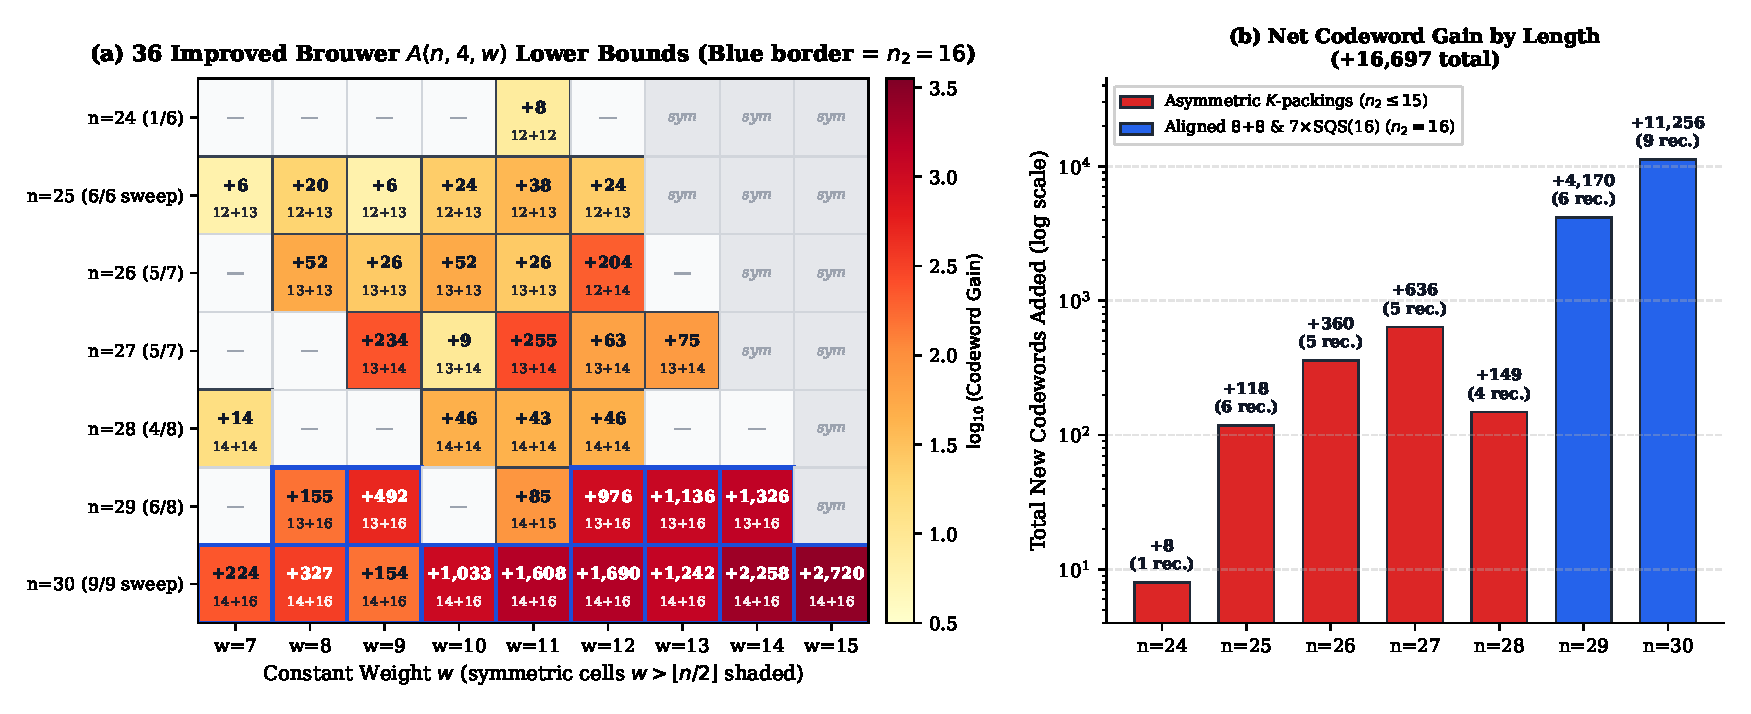
\includegraphics[width=\textwidth]{fig_bt011_frontier_heatmap.pdf}
\caption{Global frontier sweep across Andries~E.\ Brouwer's live November~24, 2026 (\texttt{22:50 CET}) $A(n, 4, w)$ table~\cite{BrouwerAndw}. (a)~Complete discovery heatmap for $24 \le n \le 30$, $7 \le w \le 15$, annotating every beaten cell with its exact codeword gain and coordinate split (blue borders denote our newly unlocked $n_2 = 16$ splits $13{+}16$ and $14{+}16$). Both $n = 25$ ($6/6$) and $n = 30$ ($9/9$) are completely swept. (b)~Aggregate codeword gain per block length ($+16{,}697$ total), illustrating the order-of-magnitude leap at $n = 29$ ($+4{,}170$) and $n = 30$ ($+11{,}256$).}
\label{fig:heatmap}
\end{figure*}

\begin{figure*}[t]
\centering
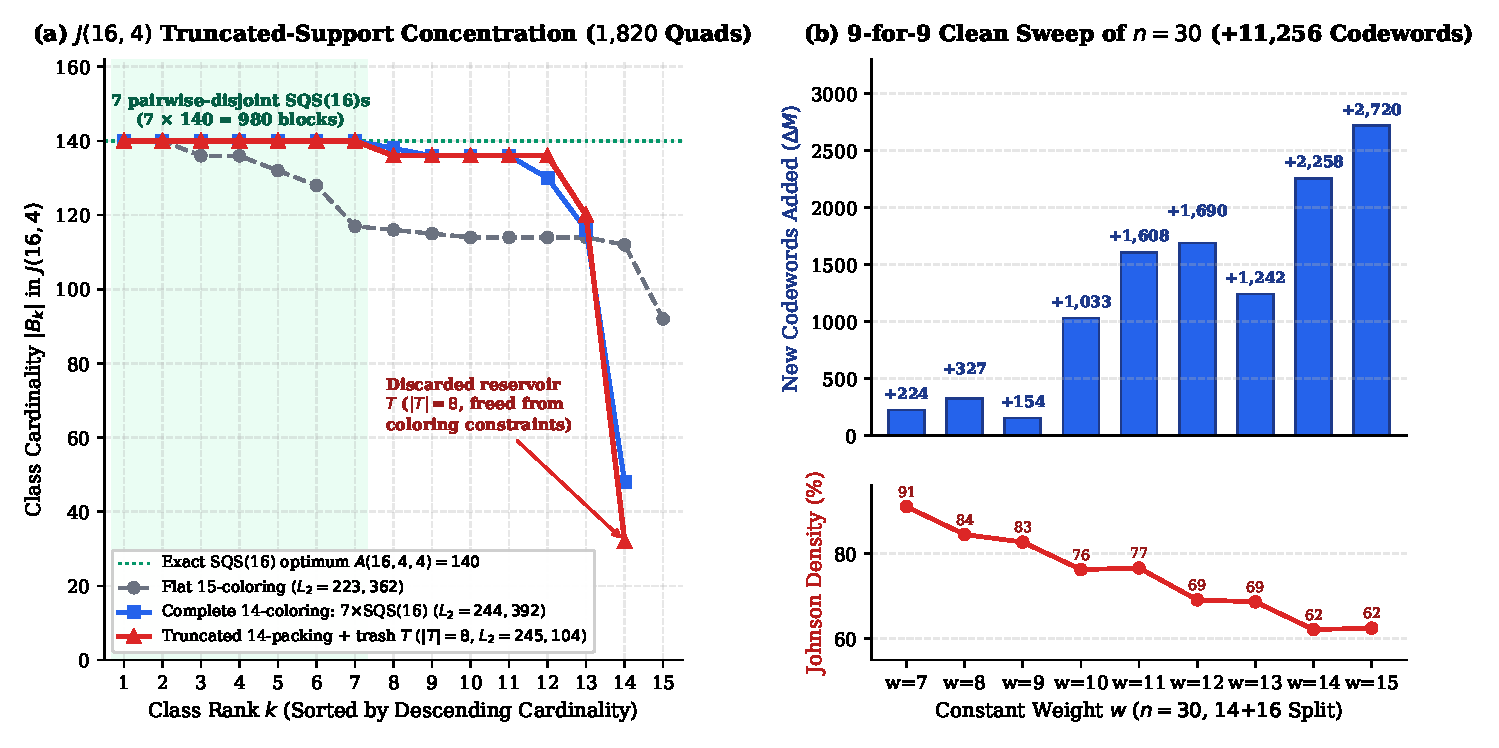
\includegraphics[width=\textwidth]{fig_bt011_asymmetric_and_sqs16.pdf}
\caption{Mechanism of the $n = 16$ breakthrough. (a)~Descending class-size spectra on $J(16, 4)$ ($1{,}820$ quadruples): releasing just $|T| = 8$ vertices into the unconstrained discarded reservoir $T$ lifts the flat $15$-coloring ($L_2 = 223{,}362$) to seven pairwise-disjoint $\mathrm{SQS}(16)$s ($140^{\times 7}$) plus five size-$136$ classes ($L_2 = 245{,}104$), alongside a complete $14$-coloring ($140^{\times 7}, 138, 136^{\times 3}, 130, 116, 48$, $L_2 = 244{,}392$). (b)~Per-weight codeword gains ($+154$ to $+2{,}720$) and Johnson-bound densities across our complete $9/9$ clean sweep of $n = 30$ ($w = 7..15$).}
\label{fig:sqs16}
\end{figure*}

\TableCleanSweepSummary
\TableAllThirtySixRecords
\TableTwentyComponents

\paragraph{Highlights of the Frontier Sweep.}
\begin{itemize}[leftmargin=1.5em,itemsep=1.5pt]
    \item \textbf{Complete 9-for-9 Clean Sweep of $n = 30$ ($w = 7..15$, $+11{,}256$ codewords):} Every single open weight at $n = 30$ is improved via the even-weight $14{+}16$ split, culminating in $A(30, 4, 15) \ge 5{,}699{,}800$ ($+2{,}720$), $A(30, 4, 14) \ge 5{,}315{,}657$ ($+2{,}258$), $A(30, 4, 12) \ge 3{,}145{,}679$ ($+1{,}690$), and $A(30, 4, 11) \ge 1{,}979{,}156$ ($+1{,}608$).
    \item \textbf{Six Records at $n = 29$ ($+4{,}170$ codewords):} Five cells ($w = 8, 9, 12, 13, 14$) leap via $13{+}16$ (peaking at $A(29,4,14) \ge 2{,}872{,}206$, $+1{,}326$), while $A(29, 4, 11) \ge 1{,}266{,}111$ ($+85$) combines two new asymmetric $n_2 = 15$ packings (\texttt{asym\_15\_6\_K13\_unif\_op4.json} and \texttt{asym\_15\_7\_K13\_14\_4dt.json}) in the $14{+}15$ split.
    \item \textbf{Complete 6-for-6 Clean Sweep of $n = 25$ ($w = 7..12$, $+118$ codewords) and Broad Gains Across $n \in \{24, 26, 27, 28\}$ ($+1{,}153$ codewords):} Driven purely by asymmetric $K$-packings on $J(12, 5)$, $J(13, 5)$, $J(13, 6)$, $J(14, 5)$, and $J(14, 6)$ plus our improved \texttt{part14.7} $L_2$-norm partition, highlighted by $A(27,4,11) \ge 518{,}269$ ($+255$), $A(27,4,9) \ge 188{,}795$ ($+234$), $A(26,4,12) \ge 402{,}141$ ($+204$), and $A(24,4,11) \ge 118{,}430$ ($+8$).
\end{itemize}

\paragraph{Live Baseline Integrity (November~24, 2026).}
The baseline oracle \url{https://aeb.win.tue.nl/codes/Andw.html} was fetched live twice on November~24, 2026 (latest snapshot \texttt{22:50 CET}, archived at \texttt{corpora/\allowbreak Andw\_live\_\allowbreak 2026\_11\_24.html}, SHA-256 \texttt{b61b7b737cd1dacc...}, full digest in \texttt{manifest.json}). Diff inspection confirmed zero changes to any $d = 4$ entry (only $A(40,8,8)$ and $A(41,10,8)$ changed on Nov~24). All $36$ beaten cells retained their original Brouwer--Etzion `\texttt{p}' lower bounds.

\section{Native Lean 4.33.0 Mechanization of the Construction Theorem}
\label{sec:lean}

Lean~4.33.0~\cite{deMouraUllrich2021Lean4} checks the distance lemmas behind Theorem~\ref{thm:asym_bsss}: weight and distance additivity, the parity law, complementation, and validity of the matched product on partial packings. The source file \texttt{BT011\_AsymmetricBSSS.lean} (included in both submission bundles; SHA-256 \texttt{5cac3dae1b7952df...}) imports only \texttt{Init}, with \textbf{zero \texttt{sorry}} and \textbf{zero custom axioms}. These lemmas do not inspect the $36$ codes. The codes are checked in Section~\ref{sec:verification}.
\begin{itemize}[leftmargin=1.5em,itemsep=1.5pt]
    \item \textbf{Lemmas on weight and distance:} Additivity of Hamming weight (\texttt{hweight\_\allowbreak append}) and distance (\texttt{hdist\_\allowbreak append}), symmetry (\texttt{hdist\_\allowbreak comm}), positivity, triangle weight bound, exact parity identity $(w_a + w_b + d_H(a,b)) \bmod 2 = 0$, equal-weight $d_H \ge 2$, weight-gap $d_H \ge 2$, and bitwise complement isometry (\texttt{bcomp\_length}, \texttt{hweight\_bcomp}, \texttt{hdist\_bcomp}).
    \item \textbf{\texttt{matched\_product\_valid}:} Any two \texttt{DisjointCWCFamily} structures $\mathcal{A}$ on $(n_1, w_1, K)$ and $\mathcal{B}$ on $(n_2, w_2, K)$, with arbitrary uncolored complements outside $\bigcup_{k<K} B_k$, yield a \texttt{ValidCWC} $(n_1 + n_2, 4, w_1 + w_2)$.
    \item \textbf{\texttt{cross\_split\_dist4}:} $d_H(u_1 \mathbin{\Vert} v_1, u_2 \mathbin{\Vert} v_2) \ge 4$ for distinct same-parity splits.
    \item \textbf{\texttt{comp\_family\_valid}:} Complement invariance $(n, w, K) \mapsto (n, n-w, K)$.
\end{itemize}
The same file also contains \texttt{bt011\_thirtysix\_records\_strictly\_beat\_nov24\_brouwer}, a kernel \texttt{decide} on $36$ hardcoded integers. It checks only that the sizes printed in Table~\ref{tab:all36} satisfy $M > \mathrm{LB}_{\mathrm{Nov24}}$ and that the printed totals are $16{,}697$ new codewords, $38{,}467{,}121$ codewords, and $486{,}375{,}836$ subtuples. That check is bookkeeping. It is not evidence that the codes exist.

Running \texttt{lean BT011\_AsymmetricBSSS.lean} on Lean~4.33.0 (\texttt{aarch64-unknown-linux-gnu}) exits with code $0$ and zero warnings. The distance lemmas depend only on the standard kernel axioms:
\begin{lstlisting}
'BT011.matched_product_valid' depends on axioms: [propext, Classical.choice, Quot.sound]
'BT011.cross_split_dist4' depends on axioms: [propext, Classical.choice, Quot.sound]
'BT011.comp_family_valid' depends on axioms: [propext, Classical.choice, Quot.sound]
\end{lstlisting}

\section{Dual Zero-Shared-Code Exact Verification and Reproducibility}
\label{sec:verification}

Because $38{,}467{,}121$ binary codewords encompass $59{,}457{,}831{,}606{,}244$ unordered pairs (impossible to test via naive $O(M^2)$ loops for $M \approx 5.7 \times 10^6$), our verification relies on an exact linear-time equivalence:

\begin{theorem}[Exact $O(wM)$ Subtuple-Uniqueness Criterion for $d_H \ge 4$]
\label{thm:subtuple}
Let $\mathcal{C} \subset \binom{[n]}{w}$ be a set of $M$ distinct binary vectors of exact Hamming weight $w$. Then
\[
\min_{u \neq v \in \mathcal{C}} d_H(u, v) \ge 4 \iff \text{all } wM \text{ deleted } (w{-}1)\text{-subsets } \big\{ u \setminus \{i\} : u \in \mathcal{C},\; i \in u \big\} \text{ are pairwise distinct.}
\]
\end{theorem}

\begin{proof}
For distinct $u, v \in \binom{[n]}{w}$, $d_H(u, v) = 2w - 2|u \cap v| \in \{2, 4, \dots, 2w\}$. Thus $d_H(u, v) < 4 \iff d_H(u, v) = 2 \iff |u \cap v| = w - 1 \iff u \cap v$ is a common $(w{-}1)$-subset of both $u$ and $v$.
\end{proof}

\begin{figure*}[t]
\centering
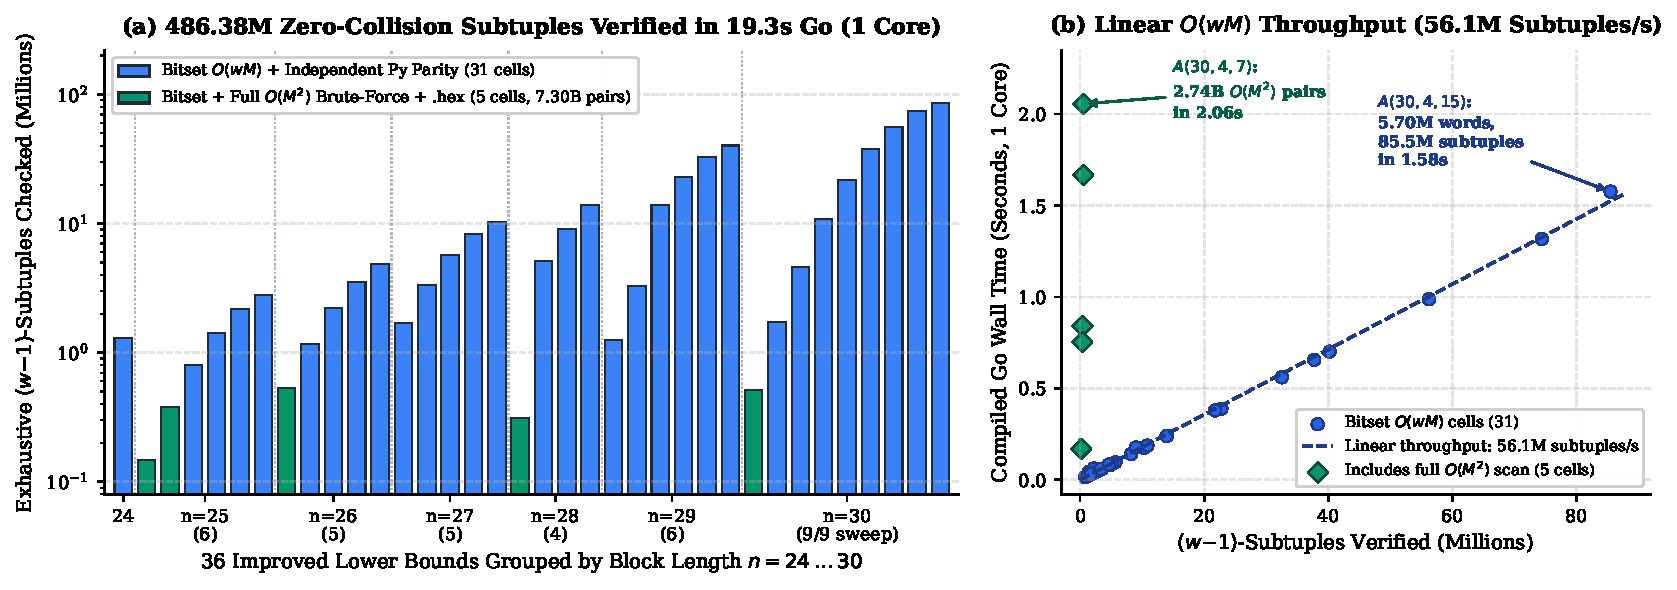
\includegraphics[width=\textwidth]{fig_bt011_verification_scale.pdf}
\caption{Exhaustive exact verification across all $36$ improved lower bounds ($38{,}467{,}121$ explicit binary codewords). (a)~Number of $(w{-}1)$-subtuples verified with zero collisions per cell ($486{,}375{,}836$ total, proving $d_H \ge 4$ across $5.946 \times 10^{13}$ pairs), highlighting the five cells additionally checked by direct $O(M^2)$ pairwise scanning ($7.30\text{B}$ pairs). (b)~Single-core Go verification time showing exact linear scaling ($56.1\text{M}$ subtuples/s, checking the $5.70\text{M}$-word code $A(30,4,15)$ in $1.58\,\mathrm{s}$).}
\label{fig:verify}
\end{figure*}

To guarantee bit-exact reproducibility across independent implementations, every component partition is canonicalized language-independently (words sorted ascending inside each class; non-empty classes sorted by $(-\text{size}, \min\text{-word})$), and every assembled code is sorted strictly ascending and hashed in fixed-width lowercase hex (\texttt{\%0<ceil(n/4)>x\char92 n}). Two completely independent verifiers (zero shared code) audited all $36$ records:
\begin{enumerate}[leftmargin=1.5em,itemsep=1.5pt]
    \item \textbf{Verifier 1 (Compiled Go Exhaustive Bitset + $O(M^2)$ Sealer, \texttt{cmd/bt011-verify-all}):} Reconstructs all $36/36$ codes ($38{,}467{,}121$ codewords) from the $20$ compact certificates + baseline corpus, verifies bit-range $0 \le c < 2^n$, exact weight $\mathrm{popcnt}(c) = w$, strict ascending distinctness, and \textbf{zero $(w{-}1)$-subset collisions across all $486{,}375{,}836$ subtuples} using an exact colex-ranked bitset (requiring only $\binom{30}{14}/8 = 18.18\,\mathrm{MB}$ RAM for $n = 30, w = 15$), finishing in \textbf{$19.3\,\mathrm{s}$ on $1$ CPU core} (Figure~\ref{fig:verify}). For all five codes with $M \le 75{,}000$ ($A(25,4,7)$, $A(25,4,8)$, $A(26,4,8)$, $A(28,4,7)$, and $A(30,4,7)$), it additionally exports explicit sorted \texttt{.hex} files and runs direct $O(M^2)$ pairwise distance scanning across all \textbf{$7{,}300{,}834{,}283$ pairs}.
    \item \textbf{Verifier 2 (Zero-Shared-Code Pure-Python Verifier, \texttt{verify\_\allowbreak bt011\_\allowbreak standalone.py}):} Independently parses every \texttt{.pk} and \texttt{.json} file via \texttt{itertools.combinations} colex generation, independently checks all \textbf{$120$ component partitions} for zero intra-class $(w{-}1)$-collisions and strict disjointness, re-assembles all $36/36$ full codes ($38{,}467{,}121$ words), runs direct full-code $(w{-}1)$-subset collision checks on all $15$ records with $M \le 250{,}000$ ($18{,}464{,}010$ subtuples), validates all $5$ exported \texttt{.hex} files byte-for-byte, and asserts \textbf{$36/36$ exact SHA-256 match ($\mathrm{Go} = \mathrm{Python}$)} in $27.17\,\mathrm{s}$.
\end{enumerate}
Both verifiers agree to the last hex digit on the global WOF-1 composite archive digest (SHA-256 over the $36$ lines \texttt{<cell>:<size>:<codewords\_sha256>\char92 n}):
\begin{center}
\texttt{\small ff6475f8763defd1c1c68935391b682d263dd09c14bc0737d7754d3bbd02a8f6}
\end{center}

\section{Honest Scope Boundaries and Open Problems}
\label{sec:scope}

\begin{enumerate}[leftmargin=1.5em,itemsep=2pt]
    \item \textbf{Boundary of Brouwer's $d = 4$ Table ($n \le 30$):} Andries~E.\ Brouwer's live \texttt{Andw.html} table~\cite{BrouwerAndw} tabulates $A(n, 4, w)$ for $w \ge 6$ only up to $n = 30$ (at $n = 31, 32$, only exact values for $w = 3, 4$ appear). Extending our aligned $8{+}8$ and $16{+}16$ product partitions to $n = 31, 32$ is immediate once public reference tables for $n \ge 31, w \ge 6$ are standardized.
    \item \textbf{Algebraic $8$-$\mathrm{SQS}(16)$ seeds, left unrun:} Etzion and Hartman~\cite{EtzionHartman1991} give $D(16) \ge 8$. We did not seed the packer with such a family. The deferral is scope. An $8$-pack would freeze eight classes at size $140$ and leave a residual packing of the remaining classes on their complement, which is a different search from the joint unseeded optimization of Section~\ref{sec:n16}. We report no measurement of that residual search. Separately, the flat $8{+}8$ partition of $J(16, 6)$ is locally rigid (every vertex has $\mathrm{deg}[u][c] \ge 4$ in every foreign class); multi-vertex Kempe moves on that partition are also unrun.
    \item \textbf{Self-Contained Verification Bundle:} The accompanying archive \texttt{bt011\_\allowbreak brouwer\_\allowbreak certificates.\allowbreak tar.gz} bundles all $20$ new compact component certificates ($\approx 360\,\mathrm{KB}$), \texttt{ls13\_\allowbreak ls15.json}, the $42$ referenced Brouwer 2010 \texttt{.pk} baselines, the $5$ explicit \texttt{.hex} codeword files ($M \le 75{,}000$), \texttt{BT011\_\allowbreak AsymmetricBSSS.lean}, and \texttt{verify\_\allowbreak bt011\_\allowbreak standalone.py}, allowing any referee to reproduce and verify all $36$ codes ($38{,}467{,}121$ codewords) from scratch in under $30\,\mathrm{s}$ using standard Python~3.
\end{enumerate}

\paragraph{Acknowledgments and Discovery Platform.}
This research was supported by Calera Labs. The Volumetric Lattice Network (VLN) workflow orchestrated the frontier audit, Johnson-graph local-search runs, Lean~4 mechanization, and certificate packaging. All mathematical constructions, compact component certificates, Lean~4 proofs, and independent verifiers are completely self-contained and require no proprietary software to verify.

{\small
\bibliographystyle{unsrt}
\bibliography{references}
}

\end{document}
